\subsection{Tipo de entidad Asignatura}

   \begin{description}

   \item[Definición] Se refiere al objeto del mundo real: \emph{``Materia que
   forma parte del plan de estudios de una titulación''}.

   \item[Características] La entidad presenta las siguientes características:
      \begin{itemize}
         \item \textbf{Nombre:} Asignatura.
         \item \textbf{Tipo:} Débil por identificación con respecto a Titulación.
         \item \textbf{Número de atributos:} 6 propios y 2 heredados.
         \item \textbf{Atributo/s identificador/es principal/es:} id\_centro junto con \\id\_titulación e id\_asignatura.
         \item \textbf{Atributo/s identificador/es alternativo/s:} id\_centro junto con \\id\_titulación y nombre\_asignatura.
         \item \textbf{Atributo/s heredado/s:} id\_centro e id\_titulación del
         tipo de entidad Titulación.
      \end{itemize}

   \item[Diagrama] La figura \ref{diagramaAsignatura} muestra el diagrama de la entidad.
   \item \begin{figure}[!ht]
            \begin{center}
            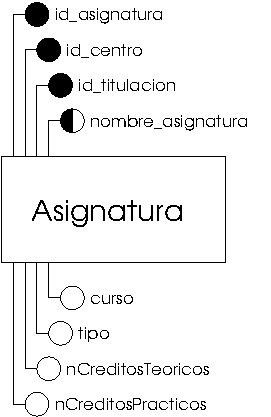
\includegraphics[]{07.Modelo_Entidad-Interrelacion/7.2.Analisis_Entidades/diagramas/asignatura.pdf}
            \caption{Diagrama de la entidad Asignatura.}
            \label{diagramaAsignatura}
            \end{center}
         \end{figure}

   \item[Descripción de los atributos propios] La entidad presenta los
   siguientes atributos propios:

   \begin{itemize}
   \item \textbf{id\_asignatura}
      \begin{itemize}
         \item \textbf{Definición:} Código que sirve como número identificativo
         para cada asignatura dentro del sistema.
         \item \textbf{Dominio:} Números naturales.
         \item \textbf{Carácter:} Obligatorio.
         \item \textbf{Ejemplo práctico:} 17.
         \item \textbf{Información adicional:} El dato lo proporciona el sistema, cuando el administrador, principal o de centro, introduce la asignatura en el sistema. Es la clave primaria junto con id\_centro y con id\_titulación.
      \end{itemize}
   \item \textbf{nombre\_asignatura}
      \begin{itemize}
         \item \textbf{Definición:} Denominación de una asignatura dentro del sistema.
         \item \textbf{Dominio:} Conjunto de caracteres alfanuméricos.
         \item \textbf{Carácter:}  Obligatorio.
         \item \textbf{Ejemplo práctico:} Lenguajes de Inteligencia Artificial.
         \item \textbf{Información adicional:} El dato lo proporciona el administrador, principal o de
         centro, en el momento de introducir la asignatura en el sistema. Es la clave alterna junto con
         id\_centro y con id\_titulación.
      \end{itemize}
   \item \textbf{curso}
      \begin{itemize}
         \item \textbf{Definición:} Nivel académico de la asignatura en una titulación.
         \item \textbf{Dominio:} Números naturales.
         \item \textbf{Carácter:}  Opcional.
         \item \textbf{Ejemplo práctico:} 2.
         \item \textbf{Información adicional:} El dato lo proporciona el administrador, principal o de
         centro, en el momento de introducir la asignatura en el sistema.
      \end{itemize}
   \item \textbf{tipo}
      \begin{itemize}
         \item \textbf{Definición:} Clasificación de la asignatura según su tipo.
         \item \textbf{Dominio:} Uno de los valores: Troncal, Obligatoria, Optativa o Libre Configuración.
         \item \textbf{Carácter:}  Opcional.
         \item \textbf{Ejemplo práctico:} Optativa.
         \item \textbf{Información adicional:} El dato lo proporciona el administrador, principal o de
         centro, en el momento de introducir la asignatura en el sistema.
      \end{itemize}
   \item \textbf{nCréditosTeóricos}
      \begin{itemize}
         \item \textbf{Definición:} Valor relacionado con el número de horas que se estima necesario para dedicar al contenido teórico de una asignatura.
         \item \textbf{Dominio:} Números reales positivos.
         \item \textbf{Carácter:}  Opcional.
         \item \textbf{Ejemplo práctico:} 3.0.
         \item \textbf{Información adicional:} El dato lo proporciona el administrador, principal o de
         centro, en el momento de introducir la asignatura en el sistema.
      \end{itemize}
   \item \textbf{nCréditosPrácticos}
      \begin{itemize}
         \item \textbf{Definición:} Valor relacionado con el número de horas que se estima necesario para dedicar al contenido práctico de una asignatura.
         \item \textbf{Dominio:} Números reales positivos.
         \item \textbf{Carácter:}  Opcional.
         \item \textbf{Ejemplo práctico:} 1.5.
         \item \textbf{Información adicional:} El dato lo proporciona el administrador, principal o de
         centro, en el momento de introducir la asignatura en el sistema.
      \end{itemize}

   \end{itemize}

   \item[Ejemplo práctico]

   \item \begin{center}
            \begin{tabular}{ | l | l | }
            \hline
            \multicolumn{2}{ | c | }{\textbf{Tipo de entidad Asignatura}} \\
            \hline
            id\_centro & 15 \\
            \hline
            id\_titulación & 3\\
            \hline
            id\_asignatura & 17\\
            \hline
            nombre\_asignatura & Lenguajes de Inteligencia Artificial\\
            \hline
            curso & 2\\
            \hline
            tipo & Optativa\\
            \hline
            nCréditosTeóricos & 3.0\\
            \hline
            nCréditosPrácticos & 1.5\\
            \hline
            \end{tabular}
         \end{center}
   \end{description}
